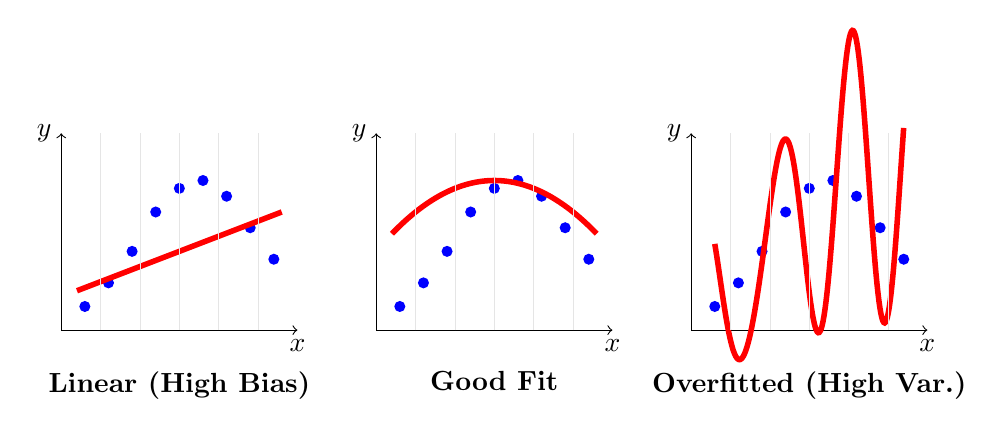
\begin{tikzpicture}[scale=1.0]
  % Subplot 1: Linear (Underfitting) - improved
  \begin{scope}[xshift=0cm]
    \draw[->] (0,0) -- (3,0) node[below] {$x$};
    \draw[->] (0,0) -- (0,2.5) node[left] {$y$};
    
    % More realistic non-linear data
    \foreach \x/\y in {0.3/0.3, 0.6/0.6, 0.9/1.0, 1.2/1.5, 1.5/1.8, 1.8/1.9, 2.1/1.7, 2.4/1.3, 2.7/0.9} {
      \fill[blue] (\x, \y) circle (2pt);
    }
    
    % Linear fit - clearly inadequate
    \draw[thick, red, line width=2pt] (0.2, 0.5) -- (2.8, 1.5);
    \node[below] at (1.5, -0.4) {\textbf{Linear (High Bias)}};
    
    % Grid
    \foreach \x in {0.5,1,1.5,2,2.5} {
      \draw[very thin, gray!20] (\x, 0) -- (\x, 2.5);
    }
  \end{scope}
  
  % Subplot 2: Good fit - improved
  \begin{scope}[xshift=4cm]
    \draw[->] (0,0) -- (3,0) node[below] {$x$};
    \draw[->] (0,0) -- (0,2.5) node[left] {$y$};
    
    % Same data points
    \foreach \x/\y in {0.3/0.3, 0.6/0.6, 0.9/1.0, 1.2/1.5, 1.5/1.8, 1.8/1.9, 2.1/1.7, 2.4/1.3, 2.7/0.9} {
      \fill[blue] (\x, \y) circle (2pt);
    }
    
    % Better polynomial fit
    \draw[thick, red, line width=2pt, domain=0.2:2.8, samples=100] plot (\x, {-0.4*(\x-1.5)^2 + 1.9});
    \node[below] at (1.5, -0.4) {\textbf{Good Fit}};
    
    % Grid
    \foreach \x in {0.5,1,1.5,2,2.5} {
      \draw[very thin, gray!20] (\x, 0) -- (\x, 2.5);
    }
  \end{scope}
  
  % Subplot 3: Overfitted - more realistic
  \begin{scope}[xshift=8cm]
    \draw[->] (0,0) -- (3,0) node[below] {$x$};
    \draw[->] (0,0) -- (0,2.5) node[left] {$y$};
    
    % Same data points
    \foreach \x/\y in {0.3/0.3, 0.6/0.6, 0.9/1.0, 1.2/1.5, 1.5/1.8, 1.8/1.9, 2.1/1.7, 2.4/1.3, 2.7/0.9} {
      \fill[blue] (\x, \y) circle (2pt);
    }
    
    % More realistic overfitted curve
    \draw[thick, red, line width=2pt, domain=0.3:2.7, samples=200] 
      plot (\x, {0.3 + 0.8*\x + 1.5*sin(7*\x r) + 0.5*cos(9*\x r) - 0.2*(\x-1.5)^2});
    \node[below] at (1.5, -0.4) {\textbf{Overfitted (High Var.)}};
    
    % Grid
    \foreach \x in {0.5,1,1.5,2,2.5} {
      \draw[very thin, gray!20] (\x, 0) -- (\x, 2.5);
    }
  \end{scope}
\end{tikzpicture}
